\chapter{Performance Evaluation}%
\label{eval}

This chapter, the performance of both of the networks outlined in
Chapter~\ref{implem} will be evaluated, such that their performance at playing
the game StarCraft II can be measured. The exact methodology for these tests is
described in Chapter~\ref{eval_method}.

Each section will be split into three, first evaluating the Deep Q network,
second the Convolutional network, and then finally comparing the two. The
results will mainly focus around the score achieved, which is the in-game is the
final score for the mini-game at hand, and for the Simple64 map this will
compare how the bot fairs across 100 games against various bots. For the
mini-games the overall comparison will allow comparisons with known baselines,
such that we can show how the agents stack up. For the Simple64 game where this
is not possible, it will instead focus on how the agent plays.

After this has been done for both the mini-games and the Simple64 map, the
results will compared overall to see what the advantages and disadvantages of
each network is, as well as comparing other parts of the networks such as
training time, and robustness.

Finally, before the conclusion, some of the additional parts of the trained
networks which are not directly linked to the performance of the network, but
do give insight into how the networks works will be shown. For example the
filters for the Convolutional network will be given here, as well as some
example outputs.

\section{Mini-games}

The mini-games are specific maps designed for training and testing different
skill requirements from the player. Each mini-game uses a different scoring
system, map and end goal. This makes it ideal for testing the agent on different
abilities for the agent to learn. Most of the mini-games incorporate some form
of randomness so that the agents do not learn to play using the same fixed
move-set. Because of this, the mini-games will be played 200 times with a
trained agent, and the mean and max scores will be recorded. This will allow a
suitable average to be taken, which takes into account the inherent randomness
of the mini-games.

For comparison, the results achieved by DeepMind are given in
Table~\ref{tab:deepmind}, as taken from the ``StarCraft II:\@ A New Challenge
for Reinforcement Learning'' paper.

\begin{table}[h]
    \centering
    \begin{tabular}{@{}c|c|rrrrrrr@{}}
        Agent & Metric &
        \rot{MoveToBeacon} & \rot{CollectMineralShards} &
        \rot{FindAndDefeatZerglings} & \rot{DefeatRoaches} &
        \rot{DefeatZerglingsAndBanelings} & \rot{CollectMineralsAndGas} &
        \rot{BuildMarines} \\ \midrule

        \multirow{2}{*}{Random Policy} & Mean & 1 & 17 & 4 & 1 & 23 & 12 & \textless{}1 \\
                                       & Max & 6 & 35 & 19 & 46 & 118 & 750 & 5 \\ \midrule

        \multirow{2}{*}{Random Search} & Mean & 25 & 32 & 21 & 51 & 55 & 2318 & 8 \\
                                       & Max & 29 & 57 & 33 & 241 & 159 & 3940 & 46 \\ \midrule

        \multirow{2}{*}{DeepMind Human Player} & Mean & 26 & 133 & 46 & 41 & 729 & 6880 & 138 \\
                                               & Max & 28 & 142 & 49 & 81 & 757 & 6952 & 142 \\ \midrule

        \multirow{2}{*}{StarCraft GrandMaster} & Mean & 28 & 177 & 61 & 215 & 727 & 7566 & 133 \\
                                               & Max & 28 & 179 & 61 & 363 & 848 & 7566 & 133 \\ \midrule \midrule

        \multirow{2}{*}{Atari-Net} & Best Mean & 25 & 96 & 49 & 101 & 81 & 3356 & \textless{}1 \\
                                   & Max & 33 & 131 & 59 & 351 & 352 & 3505 & 20 \\ \midrule

        \multirow{2}{*}{FullyConv} & Best Mean & 26 & 103 & 45 & 100 & 62 & 3978 & 3 \\
                                   & Max & 45 & 134 & 56 & 355 & 251 & 4130 & 42 \\ \midrule

        \multirow{2}{*}{FullyConv LSTM} & Best Mean & 26 & 104 & 44 & 98 & 96 & 3351 & 6 \\
                                        & Max & 35 & 137 & 57 & 373 & 444 & 3995 & 62
    \end{tabular}
    \caption{Scores achieved and outlined in the DeepMind ``StarCraft II:\@ A New
    Challenge for Reinforcement Learning'' paper.}%
    \label{tab:deepmind}%
\end{table}

\subsection{Deep Q Network}

Starting off with the Deep Q network, the mini-games that are to be used must
correlate with the network's state inputs. Since this network does not use an
image as the entire state input for the game, the mini-games chosen need to
relate the states that the network is designed to use. An example would be the
ability to move individual units. The Deep Q network does not yet support the
ability to move individual units since this is not in the networks available actions and
requires a much more complex actions to control individual units. This means
that the agent may perform sub-optimally in certain games.
On the other hand, due to the networks action space including actions that are
built up of multiple actions, this does also mean that in certain games the
agent has an advantage in that it can take a complicated action sequence.

Results are given in Table~\ref{tab:dqn_results}, where the mean and max score
achieved is given, as well as the number of episodes the agent was trained for
to achieve that score.

\begin{table}[h]
    \centering
    \begin{tabular}{@{}lrrr@{}}
        \toprule
        Map                         & Mean & Max  & Episode Count \\ \midrule
        MoveToBeacon                & 5    & 21   & 2000          \\
        CollectMineralShards        & 11   & 23   & 2000          \\
        FindAndDefeatZerglings      & 6    & 18   & 2000          \\
        DefeatRoaches               & 15   & 107  & 2000          \\
        DefeatZerglingsAndBanelings & 30   & 121  & 2000          \\
        CollectMineralsAndGas       & 2071 & 2814 & 1000          \\
        BuildMarines                & 11   & 61   & 1000          \\ \bottomrule
    \end{tabular}
    \caption{Results for the Deep Q Network}%
    \label{tab:dqn_results}%
\end{table}

Looking at the table above, the Deep Q agent struggles with the action space
available. Due to the way the agent needs to test all combinations of state and
actions to identify the best action sequence, the agent is limited in the amount
of actions it is able to take and as so is unable to select specific units or
specific locations to send the units to. This meant that the agent struggles
with maps that require a complex action sequence of splitting units or moving
units to specific position.

The MoveToBeacon map is an example where the agent is unable to send the units
to the beacon, if the beacon is on the corners of the quads that the agent can
select. Q-Learning requires the agent to test different actions in a state to
identify the optimal action to take. If the action space is too large than the
agent will require a huge amount of training time such that the agent takes a
possible combination of actions to the goal.

However, it is possible to see the agent performs well on the
FindAndDefeatZerglings and BuildMarines map. Because the Deep Q actions are made
of multiple smaller action sets, the agent is able to execute the complex
commands with a single action. This makes it possible for the agent to take a
given action and evaluate the action without needing a large action space.

The agent is all the cases has learnt the correct sequence of actions to be
taken for an optimal value approximation. The only limiting factor comes down
the action space available to the agent. In the CollectMineralsAndGas mini-game,
the agent has learnt to issue a command to the units to extract resources
without calling any other actions that would use up these resources. The
limiting factor is that the agent cannot create more SCV units, the units that
farm and extract resources, due to the complexity of the action space.

\subsection{Convolutional Network}

In contrast to the Deep Q network, the Convolutional network does not have to
consider the state inputs, due to the only input being the screen and mini-map
data. This is both an advantage and disadvantage for the network, as it does not
need tuning potentially, but does also mean that the network lacks the required
information to perform well in some of the mini-games. For example, some
mini-games require the usage of resource management and knowing when to spend
resources to build units or buildings. Since the current number of resources is
not shown on the screen to the agent, it is unable to make decisions based on
this and as such suffers in these mini-games.
Similarly, there is no issues with action space due to having access to the
entire game action space. This means the agent is able to move multiple units
independently, and perform many actions. However, as there is no compound
actions, it is much harder for the network to perform complex actions, which
puts it at a disadvantage in later mini-games.

As before, Table~\ref{tab:cnn_results} contains the mean and max
scores achieved, as well as the number of episodes the agent trained for.

\begin{table}[h]
    \centering
    \begin{tabular}{@{}lrrr@{}}
        \toprule
        Map                         & Mean & Max  & Episode Count \\ \midrule
        MoveToBeacon                & 26   & 32   & 1200  \\
        CollectMineralShards        & 84   & 110  & 7500  \\
        FindAndDefeatZerglings      & 32   & 53   & 70000 \\
        DefeatRoaches               & 57   & 304  & 70000 \\
        DefeatZerglingsAndBanelings & 42   & 103  & 70000 \\
        CollectMineralsAndGas       & 1110 & 2025 & 50000 \\
        BuildMarines                & 2    & 8    & 50000 \\ \bottomrule
    \end{tabular}
    \caption{Results for the Convolutional Network}%
    \label{tab:cnn_results}%
\end{table}

The scores above highlight one of the known weakness of the network. Both of the
final two mini-games depend heavily on the current resources. Since this is
never passed to the network, the agent struggles heavily in these challenges.
That is because the agent never knows the state of the current resources, and as
such can not react to it. For a player, they can see they are able to build a
new gathering unit to increase their production, or to build a new building such
that they are able to store more resources, or a second command centre to build
units even faster. Since the agent never knows how many resources it has, it is
unable to formulate the concept of ``There is enough resources to build a new
unit/building'', so it struggles massively and the end result is worse than the
random policies DeepMind show. Similarly for BuildMarines, the agent never knows
to build marines or buildings to increase the unit cap and so on. This is why
the passing of additional variables is an important addition.

On the other side, the mini-games that depend solely on the screen input do very
well. The first mini-game is able to be completed to the level of an average
human player and the best DeepMind approaches. After this, the other mini-games
are predominantly close to the values given such that any changes can mostly be
put down to hyperparameter choices, since only a small sample of values was able
to be tested, due to time constraints.

The vast difference in episode count needed to converge to a strong score in the
later mini-games can also be seen. The final two mini-games were cut short as
looking at the data showed that no or very little learning was occurring and as
such, there was no point continuing to train them. It should be noted however
that the Convolutional network is capable of running multiple instances of the
agent at the same time, before collating the scores. This means the agent was
trained for up to 10 hours, but covered many times more games in that time
period due to the simultaneous running of up to 64 games at once.

\subsection{Network comparison}

The Deep Q network was able to learn the required actions to play intelligently
on every mini-game despite the limitations of its action space. It would be
favourable to make the agent learn the entire base sequence of the smaller
action sets rather than giving an abstracted action such as build. In the
implementation of the Q-Learning action space, the agent was designed to show an
ability to learn using a deep neural network and not the complexity of its
action space. To show the agents ability to learn, the actions needed to be
simplified to a single command that would issue the sequence. For example, when
the agent calls the attack action, a sequence of actions is executed. This
includes selecting the marine units by issuing a select point on the map, a
select second point on map and then issuing the attack to the selected units.
Such complex sequences, will require a lager network and more training episodes.
If instead, the agent had a larger action space without these compound actions,
the agent may have been able to perform better in the maps it struggles with
such as the MoveToBeacon map.

However, this approach was taken for the Convolutional network, and showed the
issues with taking an approach that uses the full action space. The
convolutional network was able to play the MoveToBeacon map to the same level as
normal human players, as well as the DeepMind agents. However, it also struggled
greatly on the later mini-games, failing to learn either of the last two games
and performing worse than a random search policy. Using a compound action here
may have improved the performance greatly, but does have additional issues as it
strays away from how a normal human player must play the game. Additionally,
the issues with learning here however may not be due to the simple versus
compound action space, but instead due to the differences of input.

The Deep Q network takes input solely from additional data built up from the
\texttt{obs} object, and the Convolutional network solely takes input of screen
and mini-map data, which could also explain these differences. The screen and
mini-map data provides useful data across every map, since it is the same data
that a human would use. That said, due to the missing data such as resource and
unit counts, the agent struggles for any tasks involving them. Similarly, the
Deep Q network excels on tasks that use these values, but struggles for tasks
that require accurate positioning of the unit.

Broadly, this proves experimentally what was assumed earlier in the project;
The combining of the two input spaces, such that the agent had both
screen/mini-map data and additional information would allow the agent to perform
much better across a wider range of maps versus an agent that only has access to
either one of these inputs.

\section{The Simple64 Map}

The Simple64 map is a two-player map designed to be played until one player is
victorious, either through defeating the enemy or the timer ends with a draw.
The players are randomly placed at the top left corner or bottom right corner of
the map. The game will also randomly generate an opponent race for the agent to
play against which makes the agent face different types of opponents while
training.

There are two scoring systems in this mini-game:

\begin{itemize}
    \item The final reward: 1 for a win, -1 for loss and 0 for a draw.
    \item In-game score: accumulated score of how many building and units the
        agent has and each enemy unit killed or building destroyed.
\end{itemize}


\subsection{Deep Q Network}

The Simple64 map requires a complex sequence of actions for the agent to win a
given game. The difficulty is in the agent's diversity to adapt to the changing
real-time world. In this map, the agent will be randomly placed in the top left
or lower right corner. The agent will not be able to see the map, due to the fog
of war, and will be facing different opponents every run.

\begin{table}[h]
    \centering
    \begin{tabular}{@{}lrrrr@{}}
        \toprule
        Simple64      & Win  & Lose  & Draw & Episode Count \\
        Final Reward  & 7    & 40    & 53   & 100           \\
        \midrule
        \midrule
                      & Mean & Max  \\
        In-game Score & 5020 & 7100 \\
 \bottomrule
    \end{tabular}
    \caption{Results for Deep Q on Simple64}%
    \label{tab:dqn_simple}%
\end{table}

The agent started by losing every game played for about 15 episodes until it
began to attack the enemy and draw more often. After 100 training games, the
agent has begun to draw and win 60 percent of the games. From
Table~\ref{tab:dqn_simple}, we can see that the agent lost 40 games, tied for 53
and won 7.

The Deep Q network was able to identify the requirements for achieving a higher
score in the game. The agent had learnt the sequence of events required for a
minimal win in the mini-game:

\begin{itemize}
    \item Mine the resources to gather minerals
    \item Build barracks to start training an army
    \item Build supply depots to create more army units
    \item Issue attacking commands to a location with an enemy
\end{itemize}

The main difficulties the agent faced were with the amount of time it took to
achieve the given sequence above. If the agent built the barracks too late into
the game, then the enemy would have amounted a larger army would be able to win
the episode. Another issue is that the agent can only build a basic attacking
unit, the marine, whereas the opponent can create higher level units that
augment the strength of the army. For example, the enemy unit can create
tanks and planes. However, the agent can only create a marine due to the complex
actions required to manipulate the plane and higher level units. The tank needs
to be driven to the area and then set to attack mode. In attack mode, the tank
is unable to move and can only attack. This means that the agent would need to
learn how to control the tank and manoeuvre its placements so that it is a
viable option for attacking.

\subsection{Convolutional Network}
%TODO: Evaluate a number of games of the simple64 map under the CNN network.
%Give table of results, then a play by play of why it did good or bad across the
%games. Try not to do too much on the mini-games and then S64, since that is
%covered later.

\subsection{Network comparison}
%TODO: Compare the networks again, explain why this time one did well and one
%did badly. Maybe talk about consistency here, how often they won, how their in
%game strategies compare etc.


\section{Transfer and Curriculum Learning}
%TODO: Add a few examples of the above, and show how it changes the results.
% I.e. show a bot going from MoveToBeacon -> CollectMinerals ->
% FindAndDefeatZerglings and compare that to learning with FindAndDefeatZerglings only.
% Similarly, compare learning a/many mini-games and then the Simple64 map as
% well as only the Simple64 map.
% Compare how well it does, time to learn, etc.

First, the networks were tested on the MoveToBeacon mini-game and then the
CollectMineralShards game. These games were chosen due to the same action,
movement to a point, being used in both, but with the second game requiring the
control of two units and the target changing from a beacon to a mineral shard.

Firstly, the Deep Q agent was trained on the MoveToBeacon mini-game, before the
training was stopped and the agent was tested on the mini-game to show that the
agent had learnt the correct actions to take. The same model was then tested on
the CollectMineralShards mini-game without any training on the new map. The
agent was able to collect the shards and perform well without the need to be
retrained on the new mini-game. Scoring an average of 9, the agent performed
almost as well as it would have been trained only on the CollectMineralShards
map alone.

Similarly, the Convolutional agent was trained first on the MoveToBeacon
mini-game and then tested on CollectMineralShards. The agent managed to achieve
a score of 9 with no additional training. This is lower than a score achieved
with no training of 15 and much lower than the score achieved after training.
Next, and in a more realistic situation, a network was trained on MoveToBeacon
for 30 minutes and then on CollectMineralShards for 90 minutes. This was then
compared to a network that was trained solely on the CollectMineralShards
mini-game for 2 hours. This then gave a score of 60 with transfer learning,
compared to 21 without. Figure~\ref{fig:transfer_cnn_move} shows the relative
difference in learning. The transfer learning rolling average is offset by the
number of episodes it was trained on the MoveToBeacon mini-game, which is why it
does not start at 0.

\begin{figure}[h]
    \centering
    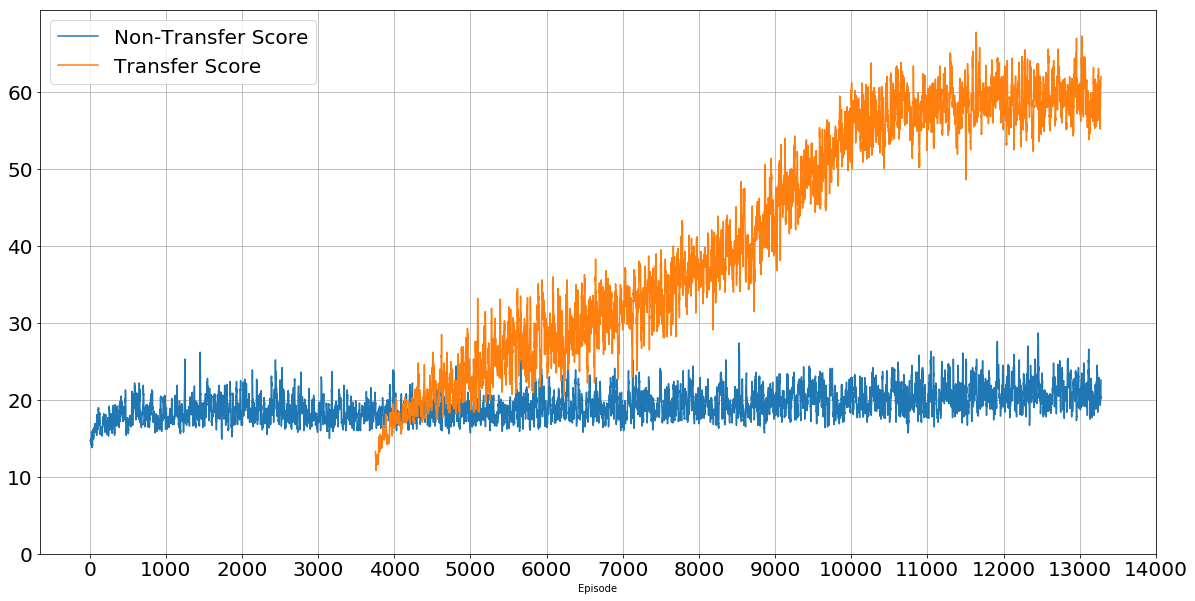
\includegraphics[width=0.97\textwidth]{cnn-transfer-move}
    \caption{Comparison of the rolling average achieved for the Transfer and
    Non-transfer learnt models.}%
    \label{fig:transfer_cnn_move}%
\end{figure}

The Deep Q agent is then tested on its ability to attack on multiple mini-games.
The agent is trained on the FindAndDefeatZerglings mini-game. This map required
the agent to learn to search the map and kill the enemy units with little
strategy required. The agent only needed to issue the attack command to increase
the overall score. The agent is then tested on the DefeatRoaches and
DefeatZerglingsAndBanelings. Again the agent was able to show the correct
actions for the given state but with the limitation that the Deep Q agent is
unable to control individual units. This is a necessary skill to achieving a
higher score on these games as the agent needs to split the units and surround
the enemies. The overall performance is similar to the agent being trained on
each of the individual mini-games.

The Deep Q network uses a negative reward function to make the agent try to
minimize the negative reward it achieves. This makes the agent likely to reduce
the expected value of a wrong action. If the agent is given a 0 for each action
that does not return a reward then the agent will tend to take those actions
more often. A negative reward reduces this behaviour but at the cost of the
values being reduced for every incorrect action taken. This increases the
difficulty of teaching an agent specific skills using curriculum learning. The
agent performs well with curriculum learning that has distinct different states.
Otherwise the agent confuses the states and actions. Below are the maps that the
agent can use curriculum learning to get the right actions without affecting the
other weights:

\begin{itemize}
    \item MoveToBeacon
    \item BuildMarines
    \item FindAndDefeatZerglings
    \item CollectMineralShards
\end{itemize}

The mini-games above provide different state and action requirements that the
agent can benefit from training on separately without reducing the weights of
other actions. When the agent is trained on one of these mini-games, there is
minimal impact to the rest of the weights.

The following mini-games are difficult for the network to train on due to the
overlap in state and actions:

\begin{itemize}
    \item DefeatRoaches
    \item FindAndDefeatZerglings
    \item DefeatZerglingsAndBanelings
    \item CollectMineralsAndGas
\end{itemize}

The best example is in the BuildMarines and CollectMineralsAndGas. The 2 maps
are different and require different actions be taken by the agent. In the
BuildMarines, the agent is encouraged and rewarded for creating more marines by
using up the available resources and farming more. However, the
CollectMineralsAndGas has the opposite effect. The agent is instead encouraged
to collect the resources and save them up rather than spending them to make
marine units. This means the agent is told to make units in one but is punished
in the other. The state space is also the same for the agent. In both maps the
agent has SCV units and a base with minerals around the map. The attacking maps
also have the same effect of requiring different strategies be used when
attacking the enemy units. The agent then needs to forget the previous strategy
it learnt and rewrite the weights with the new strategy. In order to avoid this
issue, the state space would need to include what type of enemy is being seen by
the agent in the state space. This will allow the agent to learn different
strategies of attacking different enemy unit types. But this would also increase
the state space.

\section{Overall comparison}

Comparing the 2 networks, we can see that the Deep Q network is able to perform
well in mini-games that do not require a large action space, due to the complex
action sequences used by the Deep Q network. The Convolutional network on the
other hand is able to deal with games that have a large action space, but is
unable to easily formulate the more complex strategies needed for the later
mini-games.

This means the agents perform very differently in BuildMarines versus MoveToBeacon.
The Deep Q network is able to effectively use its more complex action space in
the BuildMarines game, but falls flat when it comes to the precise spatial
ability needed for the MoveToBeacon mini-game.

The Deep Q network also trains slower due to the single instance learning of the
value approximator. The agent needs to test different actions to find the
optimal value for a given state by playing the state multiple times. The Actor
Critic method used in the Convolutional network means that we can test different
instances of models being trained before combining the results. This allows many
instances of the game to be run at once, making training quicker. However, due
to the much larger action space and the lack of compound actions, the
Convolutional network does end up taking many more episodes to reach a strong
example.

Finally, it should be mentioned how the two networks compared to the published
scores. The MoveToBeacon game is the only game where the Convolutional network
matches the published DeepMind scores. After this, the scores are in a similar
range for the most part, but do not match them exactly. As explained previously,
this is most likely due to the difference in hyperparameters and also in
training time. The network was able to beat the human player at the
DefeatRoaches mini-game however. The Deep Q network was able to beat the
DeepMind scores for the BuildMarines mini-game, however both DeepMind and our
agents were drastically under either the human or professional players score.
That said, the Deep Q network was able to beat the Random Search policy, where
the Convolutional network did not.

\section{Network Information}
%TODO: Other additional parts of the network that hasn't been covered yet but
%wasn't applicable to the implem section. CNN - Filter displays etc. DQN - could
%we see how the QTable changes? etcetc

Figures~\ref{fig:dqn-scores-1} and~\ref{fig:dqn-scores-2} show the Deep Q score
during training. We can see the score dip as the epsilon value is reduced due to
the epsilon decay. The agent then learns the correct action to take in a given
state.

Figures~\ref{fig:cnn-filter1} and~\ref{fig:cnn-filter2} show the output of the
combined convolutional layer that is used to generate the spatial actions. The
images are given in grey scale, where the predicted best location is given in
white and gets darker the lower the probability. As can be seen, the
probability starts off very murky, with lots of noise, but after training
converges such that the only choice is moving to the target location. This can
be seen in the MoveToBeacon output as a single large point relating to the
current beacon position, and multiple small points for the CollectMineralShards
mini-game relating to the current shards.

\begin{figure}[h]
  \centering
  \begin{minipage}[b]{0.45\textwidth}
    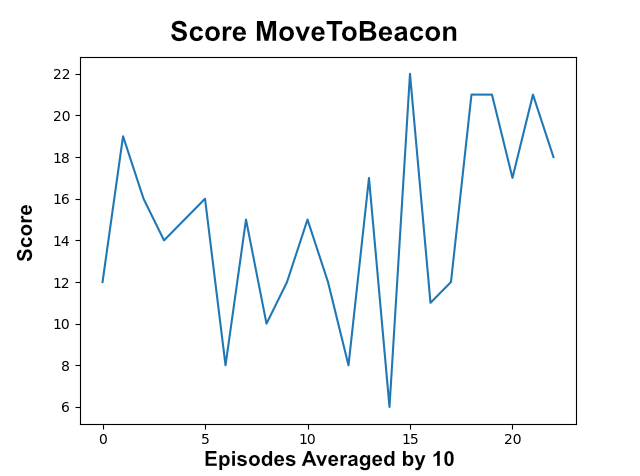
\includegraphics[width=\textwidth]{score_MoveToBeacon_train}
    \caption{Average of every 10 MoveToBeacon score during training}%
    \label{fig:dqn-scores-1}%
  \end{minipage}
  \hfill
  \begin{minipage}[b]{0.45\textwidth}
    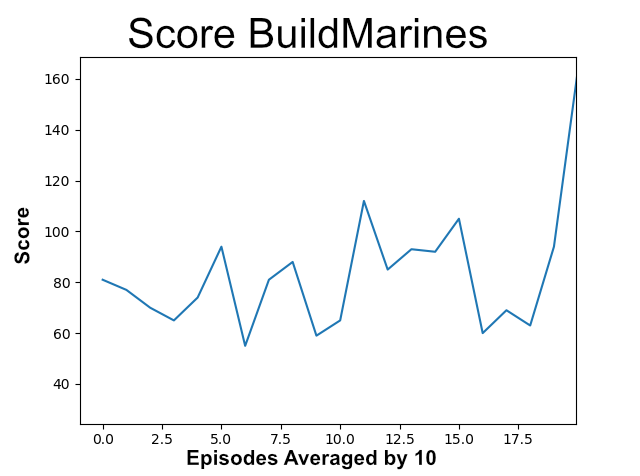
\includegraphics[width=\textwidth]{score_BuildMarines_train}
    \caption{Average score of BuildMarines runs during training, grouped over 10
    runs}%
    \label{fig:dqn-scores-2}
  \end{minipage}
\end{figure}

\begin{figure}[h]
    \centering
    \subfloat[Before training]{{
\includegraphics[width=0.45\textwidth]{Move_SmallTrain}}}%
    \subfloat[After training]{{
\includegraphics[width=0.45\textwidth]{Move_LotsOfTrain}}}%
    \caption{MoveToBeacon spatial action output before and after training.}%
    \label{fig:cnn-filter1}%
\end{figure}

\begin{figure}[h]
    \centering
    \subfloat[Before training]{{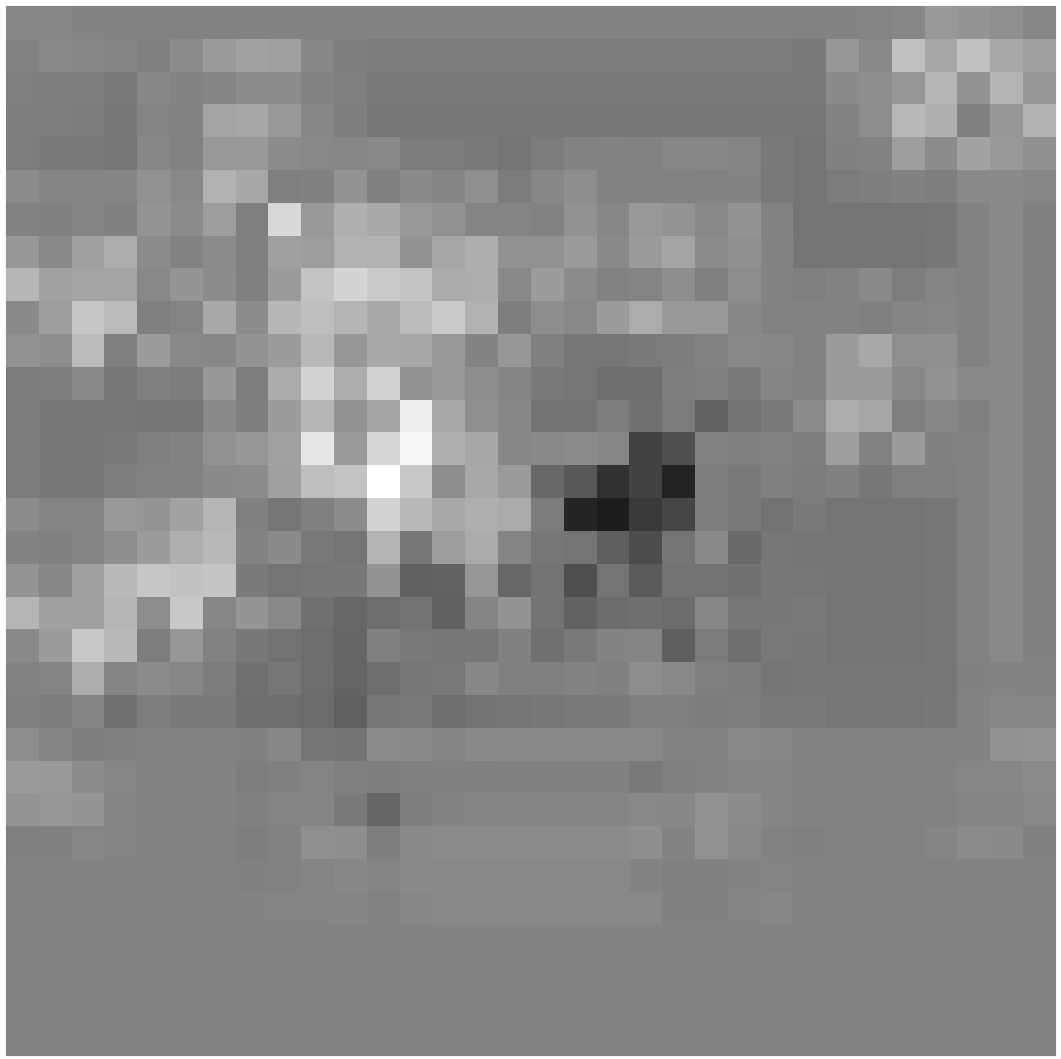
\includegraphics[width=0.45\textwidth]{Minerals_SmallTrain}}}%
    \subfloat[After training]{{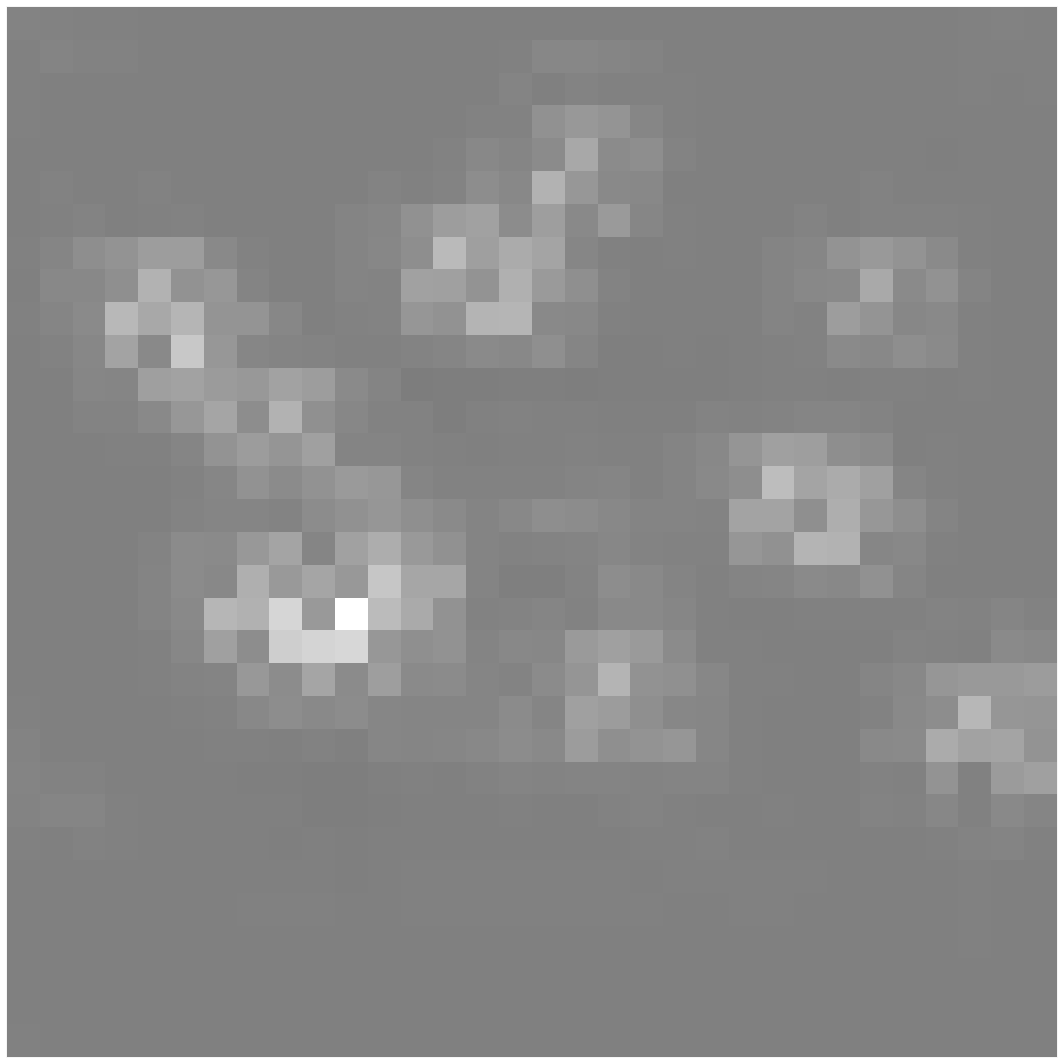
\includegraphics[width=0.45\textwidth]{Minerals_LotsOfTrain}}}%
    \caption{CollectMineralShards spatial action output before and after training.}%
    \label{fig:cnn-filter2}%
\end{figure}

\section{Conclusion}

Both networks were able to show a learning ability within each subsequent task.
They both were able to improve upon the base scores achieved at the beginning of
each training episode, and showed they were learning towards improving their
scores.  Additionally, the networks were able to learn certain behaviours from
different maps and apply the same abilities to some of the other maps.

The convolutional network required much more training time but was able to
outperform in any mini-game that required precise location based actions such as
attacking and moving the units. In comparison, the Deep Q network generally had
less time but was able to perform better in maps that require a sequence of
actions to increase the score.

However, the networks were both limited by the size of the action and input
space. When both networks were increased to allow for more information, the
networks were unable to reasonably pick up the desired outcomes. Due to the
combinational possibilities of the input and output space, the networks would
need a much longer time of training to be able to learn and achieve a reasonable
score. Additionally, the bigger the action space the harder it is for the agent
to find a smart set of actions to use.

Despite these issues, we can see that the agents were able to learn the
mini-games provided, and in some cases match  or beat the performance of a human
player in those same games.
